\section{Datenstrukturen}\label{sec:06-datenstrukturen}

\subsection{Übersicht: Laufzeiten im Vergleich}\label{sec:06-übersicht-laufzeiten-im-vergleich}
\begin{tablebox}
\begin{ZSFtable}[\ZSFfontTableDense][\ZSFtableRowStretchRoomy]{Q{1.2} Y{0.94} Y{0.93} Y{0.93}}
\toprule
\ZSFkeyword*{Datenstruktur} & \ZSFkeyword*{Suche} & \ZSFkeyword*{Einfügen} & \ZSFkeyword*{Entfernen} \\
\midrule
Liste / Array       & $\mathcal{O}(n)$          & $\mathcal{O}(n)$ \emph{(worst)}   & $\mathcal{O}(n)$ \emph{(worst)}   \\
Linked List         & $\mathcal{O}(n)$          & $\mathcal{O}(1)$ \emph{(nach Suche)} & $\mathcal{O}(1)$ \emph{(nach Suche)} \\
BST \emph{(balanciert)} & $\mathcal{O}(\log n)$ & $\mathcal{O}(\log n)$             & $\mathcal{O}(\log n)$             \\
BST \emph{(unbal.)} & $\mathcal{O}(n)$          & $\mathcal{O}(n)$                  & $\mathcal{O}(n)$                  \\
Heap                & $\mathcal{O}(n)$          & $\mathcal{O}(\log n)$             & $\mathcal{O}(\log n)$ \emph{(Top)} \\
Hash-Tabelle        & $\mathcal{O}(1)$ \emph{(erw.)} & $\mathcal{O}(1)$ \emph{(erw.)} & $\mathcal{O}(1)$ \emph{(erw.)} \\
Quadtree            & $\mathcal{O}(\log n)$ \emph{(Range)} & $\mathcal{O}(\log n)$ & --- \\
\bottomrule
\end{ZSFtable}
\end{tablebox}

\begin{statementbox}[Merke]
\begin{factlist}
\ZSFFact{Hash-Tabelle}{schnellster Zugriff im Durchschnitt, aber ungeordnet.}
\ZSFFact{BST / Heap}{geordneter Zugriff, log.\ Laufzeit — nur balanciert effizient.}
\ZSFFact{Quadtree}{spezialisiert auf 2D-Bereichs-Abfragen.}
\end{factlist}
\end{statementbox}

\subsection{Queue und Stack}\label{sec:06-queue-und-stack}
\ZSFindex{Queue}
\ZSFindex{Stack}
\ZSFindexsee{FIFO}{Queue}
\ZSFindexsee{LIFO}{Stack}
\begin{defbox}[Queue]
Eine Warteschlange, bei der Elemente nach dem \ZSFkeyword*{First In – First Out} (FIFO) Prinzip verarbeitet werden.
\begin{factlist}
\ZSFFact{\texttt{add/enqueue}}{Element am Ende der Queue einfügen}
\ZSFFact{\texttt{remove/dequeue}}{Element am Anfang der Queue entfernen}
\end{factlist}
\end{defbox}

\begin{defbox}[Stack]
Ein Stapelspeicher, der nach dem \ZSFkeyword*{Last In – First Out} (LIFO) Prinzip arbeitet.
\begin{factlist}
\ZSFFact{\texttt{add/push}}{Element oben auf den Stack legen}
\ZSFFact{\texttt{remove/pop}}{Oberstes Element entfernen}
\end{factlist}
\end{defbox}
\begin{codebox}[Stack und Queue in Python]
\begin{lstlisting}[style=CodeExpert]
stack = []  # Stapel
stack.append(x)  # push: oben drauflegen -> O(1)
top = stack.pop()  # pop: oberstes wegnehmen -> O(1)

from collections import deque  # Queue
q = deque()  # doppelt verkettete Liste (O(1) an beiden Enden)
q.append(x)  # enqueue: hinten anstellen -> O(1)
first = q.popleft()  # dequeue: vorne entnehmen -> O(1)
# list.pop(0) verschiebt alle = O(n) -> deque nutzen!
\end{lstlisting}
\end{codebox}

\begin{contentbox}[Stack: Push und Pop]
\begin{center}
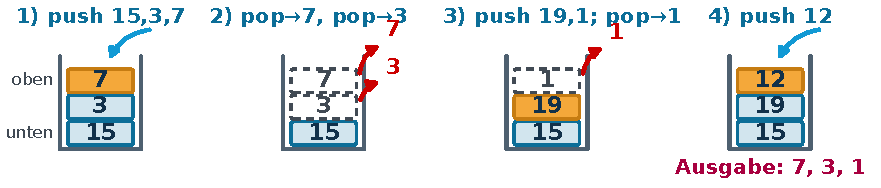
\includegraphics[width=\columnwidth]{Images/data-structure-stack-push-pop-sequence.pdf}
\end{center}
\end{contentbox}
\begin{contentbox}[Komplexitäten]
\begin{factlist}
\ZSFFact{push / pop (Stack)}{$\mathcal{O}(1)$}
\ZSFFact{enqueue / dequeue (Queue)}{$\mathcal{O}(1)$ \; (mit \texttt{deque}, nicht \texttt{list.pop(0)})}
\end{factlist}
\end{contentbox}

\subsection{Linked Lists}\label{sec:06-linked-lists}
\ZSFindex{Linked List}
\begin{defbox}[Linked List]
Elemente liegen als Knoten vor. Jeder Knoten speichert einen Wert und eine Referenz auf den nächsten Knoten.
\begin{factlist}
\ZSFFact{Vorteil}{Einfügen/Entfernen nach bekanntem Knoten ist $\mathcal{O}(1)$.}
\ZSFFact{Nachteil}{Suche nach Wert oder Position ist $\mathcal{O}(n)$.}
\end{factlist}
\end{defbox}

\begin{codebox}[Dummy-Knoten: zwei sortierte Listen mergen]
\begin{lstlisting}[style=CodeExpert]
class Node:
    def __init__(self, val, next=None):
        self.val = val
        self.next = next

def merge_sorted(a, b):
    dummy = Node(0)              # Start vor dem Ergebnis
    tail = dummy                 # letztes Element im Ergebnis

    while a is not None and b is not None:
        if a.val <= b.val:
            tail.next = a
            a = a.next
        else:
            tail.next = b
            b = b.next
        tail = tail.next

    tail.next = a if a is not None else b
    return dummy.next            # erstes echtes Element
\end{lstlisting}
\end{codebox}

\begin{contentbox}[Operationen auf einer Linked List]
\begin{center}
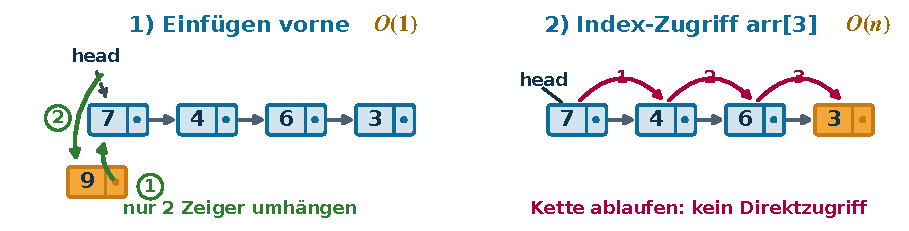
\includegraphics[width=\columnwidth]{Images/data-structure-linked-list-insert-access.pdf}
\end{center}
\end{contentbox}

\subsection{Binary (Search) Trees}\label{sec:06-binary-search-trees}
\ZSFindex[bst]{BST / Binary Search Tree}
\begin{defbox}[Binärer Suchbaum (BST)]
Für jeden Knoten gilt: Kleinere Werte stehen im linken, grössere Werte im rechten Teilbaum. Diese Regel bei jedem besuchten Knoten erneut anwenden.
\end{defbox}
\begin{contentbox}[Baumarten]
\begin{center}
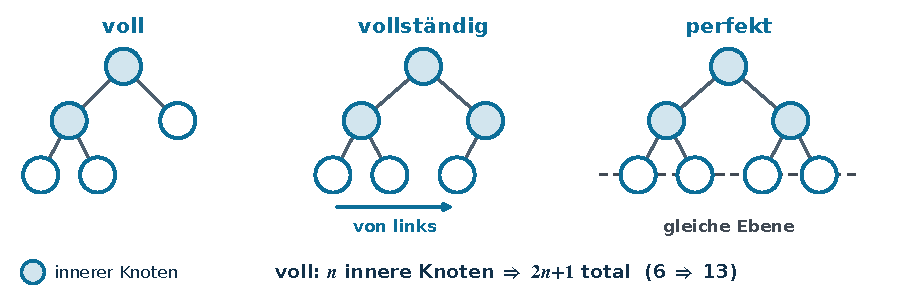
\includegraphics[width=\columnwidth]{Images/tree-full-complete-perfect-types.pdf}
\end{center}
\end{contentbox}

\begin{propertylist}[Baumtiefe bei $N$ Knoten]
\ZSFFact{Minimale Baumtiefe}{$\lceil \log_2(N + 1) \rceil$}
\ZSFFact{Maximale Baumtiefe}{$N$}
\end{propertylist}

\subsubsection{Komplexitäten}
\begin{contentbox}
\begin{factlist}
\ZSFFact{Baum aufbauen (Worst Case)}{$\Theta(n^2)$ \; (balanciert: $\Theta(n \log n)$)}
\ZSFFact{Minimum/Maximum finden}{$\mathcal{O}(n)$ \; (balanciert: $\mathcal{O}(\log n)$)}
\ZSFFact{Einfügen}{$\mathcal{O}(n)$ \; (balanciert: $\mathcal{O}(\log n)$)}
\ZSFFact{Entfernen (beliebiges Element)}{$\mathcal{O}(n)$ \; (balanciert: $\mathcal{O}(\log n)$)}
\end{factlist}
\end{contentbox}
\subsubsection{Traversierung: Baum in Liste (Pre-/In-/Postorder)}
\ZSFindex{Baumtraversierung}
\begin{codebox}[Baum in Liste umwandeln (rekursiv)]
\begin{lstlisting}[style=CodeExpert]
def preorder_list(node: Optional[Node]) -> list:
    if node is None: # Basis: leer
        return []
    return ([node.key] + preorder_list(node.left) # W->L->R
            + preorder_list(node.right))

def postorder_list(node: Optional[Node]) -> list:
    if node is None: # Basis: leer
        return []
    return (postorder_list(node.left) # L->R->W
            + postorder_list(node.right) + [node.key])

def inorder_list(node: Optional[Node]) -> list:
    if node is None: # Basis: leer
        return []
    return (inorder_list(node.left) # L->W->R
            + [node.key] + inorder_list(node.right))
\end{lstlisting}
\end{codebox}
\begin{contentbox}
\begin{center}
    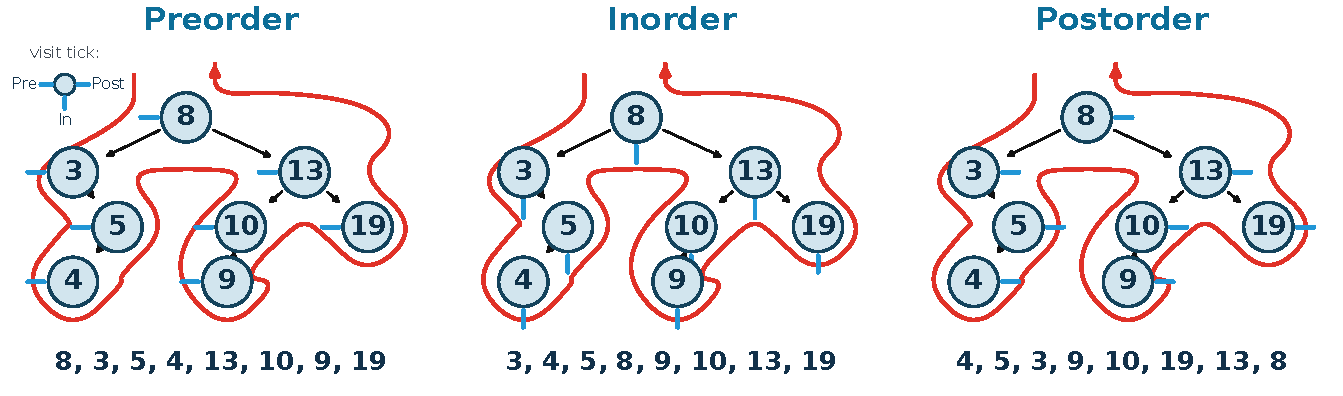
\includegraphics[width=\columnwidth]{Images/binary-tree-traversal-preorder-inorder-postorder.pdf}
\end{center}
\begin{factlist}
\ZSFFact{Preorder}{Hauptreihenfolge, damit wird der Baum gebaut}
\ZSFFact{Postorder}{Nebenreihenfolge}
\end{factlist}
\end{contentbox}

\ZSFmanualColumnBreak
\subsubsection{Knoten hinzufügen (add)}
\begin{procedure}[Einfügen auf Papier]
\ProcStep{Bei der Wurzel starten}{Neuen Wert mit dem aktuellen Knoten vergleichen.}
\ProcStep{Pfad verfolgen}{Kleiner $\rightarrow$ links, grösser $\rightarrow$ rechts.}
\ProcStep{Einfügen}{An der ersten freien Stelle einen neuen Knoten einsetzen.}
\end{procedure}
\begin{codebox}[\texttt{add()} iterativ][avg. $\Theta(\log n)$ · worst $\Theta(n)$]
\begin{lstlisting}[style=CodeExpert]
def add(self, key: int) -> bool:
    if self.root is None:  # Leerer Baum
        self.root = Node(key)
        return True  # Eingefügt
    n = self.root  # Start bei Wurzel
    while n.key != key:  # Bis Wert gefunden
        if key < n.key:  # Kleiner -> links
            if n.left is None:  # Freie Stelle
                n.left = Node(key)
                return True  # Eingefügt
            n = n.left  # Weiter absteigen
        else:  # Grösser -> rechts
            if n.right is None:  # Freie Stelle
                n.right = Node(key)
                return True  # Eingefügt
            n = n.right  # Weiter absteigen
    return False  # Wert schon vorhanden
\end{lstlisting}
\end{codebox}


\subsubsection{Knoten löschen (delete)}
\begin{procedure}[Löschen auf Papier]
\ProcStep{Kein Kind}{Knoten entfernen.}
\ProcStep{Ein Kind}{Das Kind übernimmt die Verbindung zum Elternknoten.}
\ProcStep{Zwei Kinder}{Wert durch den symmetrischen Nachfolger ersetzen und dessen alten Knoten entfernen.}
\ProcStep{Nachfolger finden}{Einmal rechts, danach so weit links wie möglich. Sein mögliches rechtes Kind übernimmt seine alte Verbindung.}
\end{procedure}
\begin{codebox}[\texttt{deleteNode()} rekursiv][bal. $\mathcal{O}(\log n)$ · worst $\mathcal{O}(n)$]
\begin{lstlisting}[style=CodeExpert]
def deleteNode(root, key):
    if root is None:  # Suchpfad endet
        return None
    if key < root.key:  # Links weitersuchen
        root.left = deleteNode(root.left, key)
    elif key > root.key:  # Rechts weitersuchen
        root.right = deleteNode(root.right, key)
    else:  # Knoten gefunden
        if root.left is None:  # Kein linkes Kind
            return root.right
        if root.right is None:  # Kein rechtes Kind
            return root.left

        # 2 Kinder: symmetrischen Nachfolger übernehmen
        successor = findMin(root.right)  # Kleinster rechts
        root.key = successor.key  # Wert ersetzen
        root.right = deleteNode(root.right, successor.key)
    return root

def findMin(node):
    while node.left is not None:  # So weit links wie möglich
        node = node.left
    return node  # Kleinster Knoten
\end{lstlisting}
\end{codebox}

\begin{contentbox}[BST: Knoten mit zwei Kindern löschen]
\begin{center}
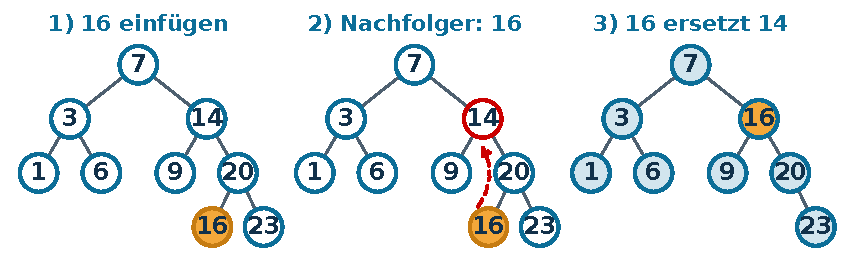
\includegraphics[width=\columnwidth]{Images/binary-search-tree-delete-two-children-successor.pdf}
\end{center}
\end{contentbox}

\subsubsection{Knoten suchen (search)}
\begin{codebox}[\texttt{search()} iterativ][avg. $\Theta(\log n)$ · worst $\Theta(n)$]
\begin{lstlisting}[style=CodeExpert]
def search(self, key: int) -> Optional[Node]:
    n = self.root  # Start bei Wurzel
    while n is not None and n.key != key:  # Bis Fund/Ende
        if key < n.key:  # Kleiner -> links
            n = n.left
        else:  # Grösser -> rechts
            n = n.right
    return n  # Knoten oder None
\end{lstlisting}
\end{codebox}
\subsection{Heaps}\label{sec:06-heaps}
\ZSFindex{Heap}
\ZSFindexsee{Max-Heap}{Heap}
\ZSFindexsee{Min-Heap}{Heap}

\subsubsection{Grundidee eines Binary Heaps}
\begin{defbox}[Binary Heap]
Ein Binary Heap ist eine vollständige Binärstruktur, bei der gilt:
\begin{factlist}
\ZSFFact{Min-Heap}{Elternknoten ist stets kleiner als seine Kinder.}
\ZSFFact{Max-Heap}{Elternknoten ist stets grösser als seine Kinder.}
\end{factlist}

Heaps werden in einer Liste gespeichert, sodass die Knotenebenen hintereinander notiert sind:
\[
\texttt{[1, 2, 3, 4, 5, 6]} \Rightarrow \text{Index: } 0,1,2,\dots
\]
\end{defbox}
\begin{center}
    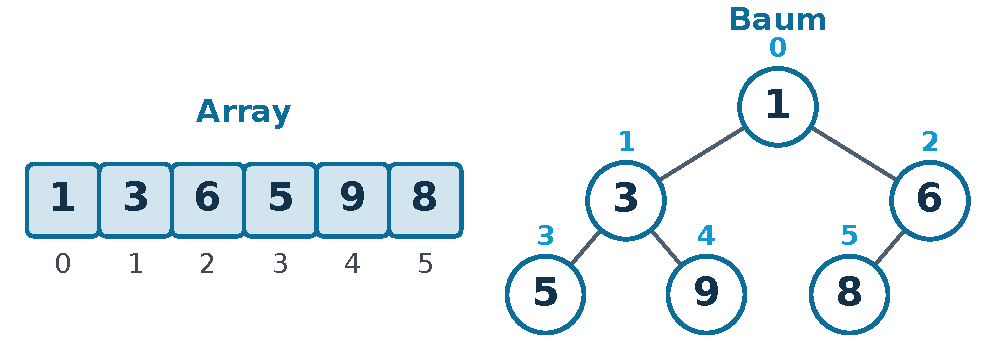
\includegraphics[width=\columnwidth]{Images/binary-heap-array-tree-index-representation.pdf}
\end{center}

\begin{contentbox}[Zugriffsformeln]
\begin{factlist}
\ZSFFact{\texttt{parent}}{$(i-1)//2$}
\ZSFFact{\texttt{left child}}{$2i + 1$}
\ZSFFact{\texttt{right child}}{$2i + 2$}
\ZSFFact{Höhe}{$\log_2(N+1)$ mit $N = \texttt{len(list)}$}
\end{factlist}
\end{contentbox}
\subsubsection{Komplexitäten}
\begin{contentbox}
\begin{factlist}
\ZSFFact{Aufbauen mit \texttt{siftUp}}{$\Theta(n \log n)$ — Elemente nacheinander einfügen}
\ZSFFact{Bottom-up-Heapify}{$\Theta(n)$ — ab letztem Elternknoten \texttt{SiftDown}}
\ZSFFact{Maximum/Minimum holen}{$\mathcal{O}(1)$}
\ZSFFact{Einfügen in Heap}{$\mathcal{O}(\log n)$}
\ZSFFact{Entfernen (Top-Element)}{$\mathcal{O}(\log n)$}
\end{factlist}
\end{contentbox}

\subsubsection{Heapify (Liste in Heap umwandeln)}
\ZSFindex{Heapify}
\begin{codebox}[Heapify: sift-up-Variante]
\begin{lstlisting}[style=CodeExpert]
def heapify(list):
    for i in range(len(list)):  # Knoten einzeln einfügen
        while list[(i - 1)//2] > list[i] and i > 0:
            swap(list, (i - 1)//2, i)  # Mit Eltern tauschen
            i = (i - 1)//2  # Beim Elternknoten weiter
    return
\end{lstlisting}
\end{codebox}
\begin{codebox}[Heapify: bottom-up-Variante]
\begin{lstlisting}[style=CodeExpert]
def heapify(list):
    n = len(list)
    # Eltern: unten rechts bis zur Wurzel
    for i in range(n//2 - 1, -1, -1):
        shift_down(list, i, n)  # Teilbaum reparieren
    return
\end{lstlisting}
\end{codebox}

\subsubsection{SiftDown (Element nach unten schieben)}
\begin{contentbox}
Beim Entfernen der Wurzel (z.\,B. Max-Element bei Max-Heap) wird das letzte Element nach oben geschoben und mit seinen Kindern verglichen. Dabei wird immer mit dem grösseren (bzw. kleineren bei Min-Heap) Kind getauscht.
\end{contentbox}
\begin{codebox}[SiftDown nach Entfernen]
\begin{lstlisting}[style=CodeExpert]
def SiftDown(a, i, m):
    while 2*i + 1 < m:  # Solange ein Kind existiert
        j = 2*i + 1  # Zuerst linkes Kind wählen
        if j + 1 < m and a[j] < a[j + 1]:
            j += 1  # Rechtes Kind ist grösser
        if a[i] >= a[j]:  # Eltern >= grösstes Kind
            break
        a[i], a[j] = a[j], a[i]  # Nach unten tauschen
        i = j  # Eine Ebene tiefer weiter
\end{lstlisting}
\end{codebox}

\begin{contentbox}[Min-Heap: Wurzel entfernen]
\begin{center}
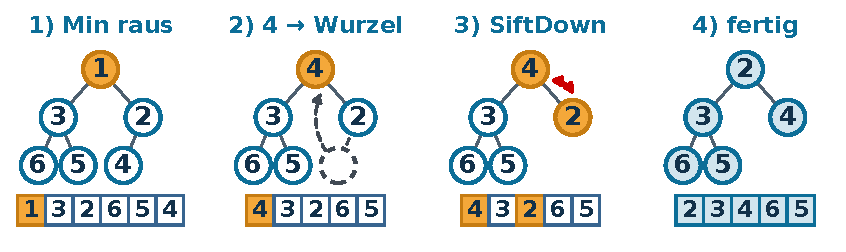
\includegraphics[width=\columnwidth]{Images/min-heap-extract-min-siftdown.pdf}
\end{center}
\end{contentbox}

\subsubsection{Sortieren mit Heaps (Heap Sort)}
\begin{codebox}[Heap Sort mit SiftDown]
\begin{lstlisting}[style=CodeExpert]
def SortHeap(a):
    heapify(a)  # Max-Heap aufbauen
    for i in reversed(range(len(a))):
        swap(a[0], a[i])  # Grössten Wert ans Ende
        SiftDown(a, 0, i)  # Restlichen Heap reparieren
    return
\end{lstlisting}
\end{codebox}

\subsubsection{Elemente einfügen und löschen}
\begin{procedure}[Einfügen auf Papier]
\ProcStep{Platz wählen}{Neuen Knoten unten an der ersten freien Stelle von links einsetzen.}
\ProcStep{Nach oben tauschen}{Min-Heap: kleinere Werte nach oben; Max-Heap: grössere Werte nach oben. Mit dem Elternknoten tauschen, solange die Reihenfolge falsch ist.}
\end{procedure}

\begin{procedure}[Top entfernen auf Papier]
\ProcStep{Wurzel ersetzen}{Wurzelwert entfernen. Wert unten ganz rechts an die Wurzel setzen und den unteren Knoten löschen.}
\ProcStep{Nach unten tauschen}{Im Min-Heap das kleinere, im Max-Heap das grössere Kind wählen. Mit diesem Kind tauschen, solange die Reihenfolge falsch ist.}
\end{procedure}

\begin{procedure}[Heap aufbauen und kontrollieren]
\ProcStep{Unten beginnen}{Bei den untersten Eltern rechts starten. Jeden Wert wie beim Entfernen nach unten tauschen. Danach Ebene für Ebene bis zur Wurzel weitergehen.}
\ProcStep{Kontrolle}{Unten sind die Knoten von links gefüllt, ohne Lücke. Jeder Elternwert steht in der richtigen Reihenfolge zu seinen Kindern.}
\end{procedure}

\begin{contentbox}[Min-Heap: Einfügen und SiftUp]
\begin{center}
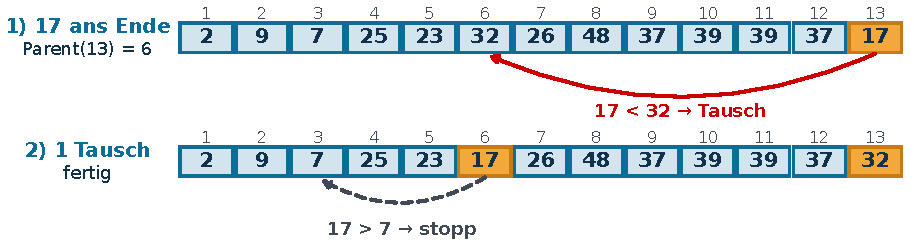
\includegraphics[width=\columnwidth]{Images/min-heap-insert-siftup-array.pdf}
\end{center}
\end{contentbox}
\begin{statementbox}[Indexierung in der Grafik]
Die Grafik zählt Positionen ab 1; die Python-Formeln oben verwenden Indizes ab 0.
\end{statementbox}
\begin{codebox}[\texttt{removeMax()}]
\begin{lstlisting}[style=CodeExpert]
def removeMax(heap):
    if len(heap) == 0:
        return None
    max_val = heap[0]  # Wurzel sichern
    heap[0] = heap[-1]  # Letzten Knoten nach oben
    heap.pop()  # Alten letzten Knoten löschen
    SiftDown(heap, 0, len(heap))  # Nach unten reparieren
    return max_val
\end{lstlisting}
\end{codebox}




\subsection{Hash-Tabellen}\label{sec:06-hash-tabellen}
\ZSFindex{Hash-Tabelle}

\subsubsection{Hash: Grundidee}
\begin{defbox}[Hash-Tabelle]
Eine Hash-Tabelle speichert ungeordnete Sammlungen \textbf{einzigartiger Elemente} (z.\,B. \texttt{set} oder \texttt{dict} in Python).

\ZSFkeyword*{Hashing}: Einer Eingabe wird mittels \ZSFkeyword*{Hash-Funktion} ein Integer zugewiesen. Die Platzierung im Array der Länge $M$ erfolgt am Index:
\[
\texttt{index} = \texttt{hash}(x)\ \%\ M \quad(\text{math: } \bmod)
\]
\end{defbox}

\subsubsection{Laufzeiten}
\begin{contentbox}
\begin{factlist}
\ZSFFact{Suche, Einfügen, Entfernen (Erwartungswert)}{$\mathcal{O}(1)$}
\ZSFFact{Suche, Einfügen, Entfernen (Worst Case)}{$\mathcal{O}(n)$}
\end{factlist}
\end{contentbox}

\subsubsection{Kollisionsbehandlung}
\ZSFindex{Kollisionsbehandlung}
\begin{contentbox}
Treffen mehrere Elemente auf denselben Index, gibt es zwei Lösungsansätze:
\begin{factlist}
\ZSFFact{Chaining}{Am Index wird der Head-Knoten einer \ZSFkeyword*{Linked List} gespeichert, die alle kollidierenden Elemente aufnimmt. \ZSFsectionref{sec:06-linked-lists}\\
  \emph{Vorteil:} Ein oft wiederholter Hash blockiert nicht die restliche Tabelle.}
\ZSFFact{Probing}{Ist der Index besetzt, wird zirkulär der nächste freie Index (\ZSFkeyword*{Wrap-around}) gesucht. \\
  \emph{Vorteil:} Alle Daten bleiben Cache-freundlich im Array. \\
  \emph{Nachteil:} Löschungen erfordern \ZSFkeyword*{Tombstoning} (spezielle Literale als Platzhalter) oder komplexes Rückwärts-Verschieben.}
\end{factlist}
\end{contentbox}

\begin{contentbox}[Lineares Probing]
\begin{center}
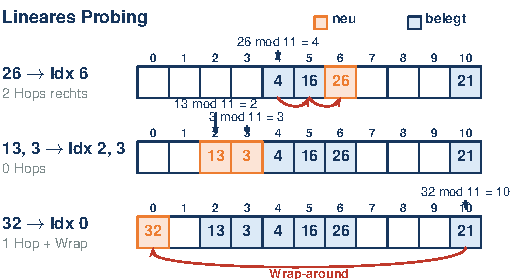
\includegraphics[width=\columnwidth]{Images/hash-table-linear-probing-collisions.pdf}
\end{center}
\end{contentbox}
\begin{codebox}[Chaining mit Buckets]
\begin{lstlisting}[style=CodeExpert]
def our_hash(word):
    return ord(word[0])           # einfache Hash-Fkt.

def create_hash_table(l, M):
    res = [[] for _ in range(M)]  # M leere Buckets
    for x in l:
        idx = our_hash(x) % M     # % statt mod!
        if x not in res[idx]:     # keine Duplikate
            res[idx].append(x)    # chaining: anhängen
    return res
\end{lstlisting}
\end{codebox}


\subsection{Quadtrees}\label{sec:06-quadtrees}
\ZSFindex{Quadtree}

\subsubsection{Quadtree: Idee \& Struktur}
\begin{defbox}[Quadtree \& Struktur]
Quadtrees sind \ZSFkeyword*{volle Quarternärbäume} ($0$ oder $4$ Kinder) zur effizienten Verarbeitung \textbf{räumlicher 2D-Daten} (z.\,B. Rechteck-Abfragen).
\begin{factlist}
\ZSFFact{$l, u$}{untere linke Ecke $l$ / obere rechte Ecke $u$}
\ZSFFact{$m$}{Maximalkapazität}
\ZSFFact{$p$}{Liste von Punkten}
\ZSFFact{$c_0..c_3$}{$4$ Kinder-Quadtrees}
\end{factlist}
\end{defbox}
\begin{codebox}[Quadtree-Knoten]
\begin{lstlisting}[style=CodeExpert]
class QuadTree:
    def __init__(self, l, u, m):
        self.l, self.u = l, u     # untere/obere Ecke
        self.m = m                # Kapazität
        self.p = []               # Punkte im Knoten
        self.c = [None]*4         # Kinder c0..c3
\end{lstlisting}
\end{codebox}

\subsubsection{Einfügen \& Split}
\begin{procedure}[Ablauf]
\ProcStep{Einfügen}{Ein Punkt wird zu $p$ hinzugefügt.}
\ProcStep{Split}{Überschreitet die Anzahl der Punkte die Kapazität $m$, wird der Knoten in \textbf{vier Viertel} partitioniert.}
\ProcStep{Aufteilen}{Die Punkte aus $p$ werden auf die Kinder aufgeteilt und das eigene $p$ geleert.}
\end{procedure}

\begin{contentbox}[Konstruktion]
\begin{center}
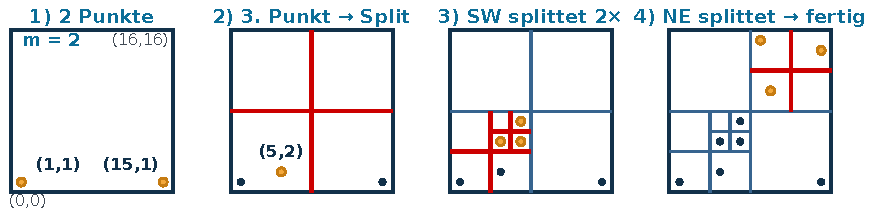
\includegraphics[width=\columnwidth]{Images/quadtree-point-insertion-splits.pdf}
\end{center}
\end{contentbox}

\begin{contentbox}[Resultierender Baum]
\begin{center}
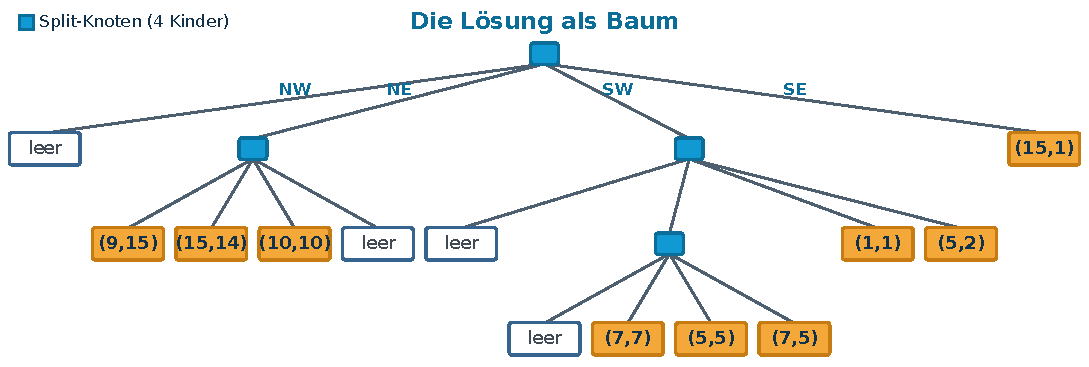
\includegraphics[width=\columnwidth]{Images/quadtree-final-tree-representation.pdf}
\end{center}
\end{contentbox}

\subsubsection{Rechtecks-Abfrage (Range Query)}
\ZSFindex{Range Query}
\begin{contentbox}
\begin{factlist}
\ZSFFact{Laufzeit}{Die Suche wächst logarithmisch mit der Anzahl der Punkte: $\mathcal{O}(\log n)$.}
\ZSFFact{Pruning}{Schneidet das Such-Rechteck einen Quadranten nicht, wird dieser Zweig \textbf{komplett ignoriert}.}
\end{factlist}
\end{contentbox}
\begin{codebox}[Quadtree: Punkte in Rechteck suchen (Range Query)]
\begin{lstlisting}[style=CodeExpert]
def query(node, q_l, q_u):  # q_l/q_u: Grenzen -> Punktliste
    if not overlaps(node, q_l, q_u):  # Pruning!
        return []                     # Zweig ignorieren
    hits = [pt for pt in node.p       # lokale Punkte
            if inside(pt, q_l, q_u)]
    for child in node.c:              # rekursiv in Kinder
        if child is not None:
            hits += query(child, q_l, q_u)
    return hits
\end{lstlisting}
\end{codebox}

\subsubsection{Wann lohnt sich ein Quadtree?}
\begin{statementbox}
Die \textbf{Konstruktion} des Baumes ist relativ aufwendig; der Einsatz lohnt sich daher erst bei \textbf{höherfrequentierten Abfragen}.
\end{statementbox}
